\documentclass[12pt]{article}
\usepackage{times}
\usepackage[titletoc]{appendix}
\usepackage{graphicx}
\usepackage{lineno}
\usepackage{multirow}
\usepackage[english]{babel}
\usepackage{hyperref}
\hypersetup{
    colorlinks=true,       % false: boxed links; true: colored links
    linkcolor=blue,          % color of internal links (change box color with linkbordercolor)
    citecolor=darkgreen,        % color of links to bibliography
    filecolor=magenta,      % color of file links
    urlcolor= black           % color of external links
}
\usepackage{typearea} 
\usepackage{amssymb}
\usepackage{amsfonts}
\usepackage{amsmath}
\usepackage{enumerate}
\usepackage[round,authoryear]{natbib}

\renewcommand{\baselinestretch}{1.2}
\newcommand{\bbar}[1]{\overline{#1}}

\usepackage{color}
	 \definecolor{darkred}{rgb}{0.75,0,0}
	 \definecolor{darkgreen}{rgb}{0,0.5,0}
	 \definecolor{darkblue}{rgb}{0,0,0.75}
\newcommand{\cha}[1]{\textcolor{darkblue}{#1}}
\newcommand{\marcus}[1]{\textcolor{darkred}{#1}}

%\newcommand{\arne}[1]{\textcolor{blue}{#1}}
%\newcommand{\cha}[1]{\textcolor{red}{#1}}
%\newcommand{\hin}[1]{\textcolor{darkred}{#1}}
%\newcommand{\AP}[1]{\textcolor{darkgreen}{#1}}

\title{\vspace*{-22mm}\bf Eco-evolutionary dynamics of mutualisms}
\author{Chaitanya S. Gokhale$^{1*}$,
Marcus Frean$^{2}$,
 \and Paul B. Rainey$^{1,3}$ \\
\normalsize $^{1}$New Zealand Institute for Advanced Study, Massey University, Auckland, New Zealand, \\
\normalsize $^2$Victoria University of Wellington, Wellington, New Zealand\\
\normalsize $^3$Max Planck Institute for Evolutionary Biology, \\
\normalsize August-Thienemann-Stra{\ss}e 2, 24306 Pl\"{o}n, Germany,\\
}

\date{}

\begin{document}

\linenumbers
\maketitle

\begin{abstract}
Mutualistic relationships pose a conundrum for evolutionary theory.
Species that exploit other species would do better than sustaining a long drawn out mutually costly relationship. However we do see mutualistic relationships amongst even the most unlikely partners \ldots.
Eco-evolutionary dynamics \ldots
\end{abstract}

\noindent
Keywords: mutualism,evolutionary game theory,multiple players

\tableofcontents

\section{Introduction}

As with many concepts, we can trace back the study of mutualism to Aristotle \citep{aristotle:book:350}.
Formally the Belgian zoologist Pierre van Beneden coined the term mutualism in $1873$ \citep{bronstein:book:2003}.
Mutualistic relationships, interspecific interactions that benefit both species, have been empirically studied for many years 
\citep{boucher:book:1985,hinton:PTENHS:1951,wilson:AmNat:1983,bronstein:QRB:1994,pierce:ARE:2002,kiers:Nature:2003,bshary:ASB:2004} and a considerable body of theory has been put forth explaining the evolution and maintenance of such relationships \citep{poulin:JTB:1995,doebeli:PNAS:1998,noe:book:2001,johnstone:ECL:2002,bergstrom:PNAS:2003,hoeksema:AmNat:2003,akcay:PRSB:2007,bshary:Nature:2008}.
Most examples of mutualisms lend themselves to the idea of direct reciprocity \citep{trivers:QRB:1971} and have thus been extensively studied using evolutionary game theory.
The interactions in these models are usually dyadic: the fundamental interaction is between two individuals, one from each species, and the sum of many such interactions determines the evolutionary dynamics.
However, in many cases interactions between species cannot be reduced to such dyadic encounters \citep{stadler:book:2008}.

For example, in the interaction between ants and aphids or butterfly larvae \citep{pierce:BES:1987,hoelldobler:book:1990} many ants tend to each of the soft bodied creatures, providing them with shelter and protection from predation and parasites, in exchange for honeydew, a rich source of food for the ants \citep{hill:OEC:1989,stadler:book:2008}.
This is a one-to-many interaction from the perspective of the larva.
Another well studied example of a one-to-many interaction is that of the plant-microbe mutualism wherein leguminous hosts prefer rhizobial symbionts that fix more nitrogen \citep{kiers:Nature:2003}, or where plants provide more carbon resources to fungal strains that are providing better access to nutrients \citep{kiers:Science:2011}.
Moving from a plant host to an animal host, a well studied example is that of the mutualistic relationship between the bioluminescent bacteria \textit{Vibrio fischeri} and \textit{Euprymna scolopes}, the bobtail squid \citep{mcfallngai:PLoSB:2014}. Numerous bacteria are hosted in the crypts of the squid's light organ, where they produce light despite it being costly. The bacteria mature and develop within the squid, however those that fail to produce bioluminescence are evicted. While the variation in the phenotypes of the interacting partners has been acknowledged, the usual analysis focuses on the interaction between the two species without addressing this additional complexity.

Identifying and quantifying the intraspecific variation can be a
daunting task \citep{behm:JE:2014}.  Intraspecific interactions are
usually studied in isolation and separate from the interspecies
relationships. \marcus{need to mention this example first} 
While the cohorts of cleaner fish together have been
taken to determine the quality of a cleaning station
\citep{bshary:AB:2002,bshary:book:2003}, this can also drive variation
of quality of cleaning within a cleaning station via
interactions of individual cleaner fish amongst themselves.  In this
manuscript we look at the broader picture of how the evolutionary
dynamics are shaped when both the inter as well as intra species
dynamics are taken together.  We find that including the full range of
interactions provides us with a set of rich and intricate dynamics
which are not possible when one of these dimensions is ignored.

Mutualistic relationships are between species by definition, and timing may be crucial for their maintenance. \marcus{this next sentence is awkward but I haven't fixed it} Hence it is natural to imagine that the observed relationship may be seasonal and the interactions as not a continuous feature of the evolutionary dynamics of a single species. In a changing ecology changes in global climate might affect the timing of the point in a season when flowers mature and when their dispersers do, quite easily disrupting delicately balanced mutualistic interactions. Unless both of the interacting species can respond in a similar fashion such a mutualism will break down \citep{warren:GCB:2014}.


We tackle this seasonality by varying the duration of the impact of intraspecies and interspecies dynamics.  \marcus{do we? not obvious where the duration enters - we have $p$ but that's not a duration.}
Furthermore to complete the ecological picture we study not just the evolutionary but the population dynamics of the mutualists.
Allowing for extinctions informs us as to the population densities we might expect to find among mutualistic interactions in nature. \marcus{??}
We demonstrate the crucial nature of the feedback between population and evolutionary dynamics which can maintain mutualisms preventing either or both species from going extinct. 
We make use of evolutionary game theory to analyze how benefits are shared between the two mutualistic species \citep{weibull:book:1995,hofbauer:JMB:1996,hofbauer:book:1998}.
Beginning with the previously studied interspecies dynamics as the foundational framework \citep{gokhale:PRSB:2012} we increase the complexity of the system by including intraspecies dynamics, population dynamics and seasonality.
The rich dynamics observed provides us with novel insights about the immense asymmetries in mutualisms and the fragility of such delicately balanced interactions.

%\marcus{This paragraph - is it about 1-1 vs 1-many, or dyadic vs ...?  Seems like it's setting up to be a ``Dyadic isn't enough'' para. In that case fine but the next para should be making the (main) point that intra-specific interactions are perhaps an important, and hitherto ignored, determinant of evolutionary outcomes for mutualisms.  }
%\cha{This was a haphazard collection of ideas. Now I have ordered them.
%\begin{itemize}
%	\item First - general mutualism
%\item Second - why we need more than dyadic
%\item Third- Why we need intra species interactions to be included and what we show in this manuscript
%\end{itemize}
%Third paragraph is way too long and I think can be shortened...have a look
%}



\section{Model and Results}


\begin{figure}
\begin{center}
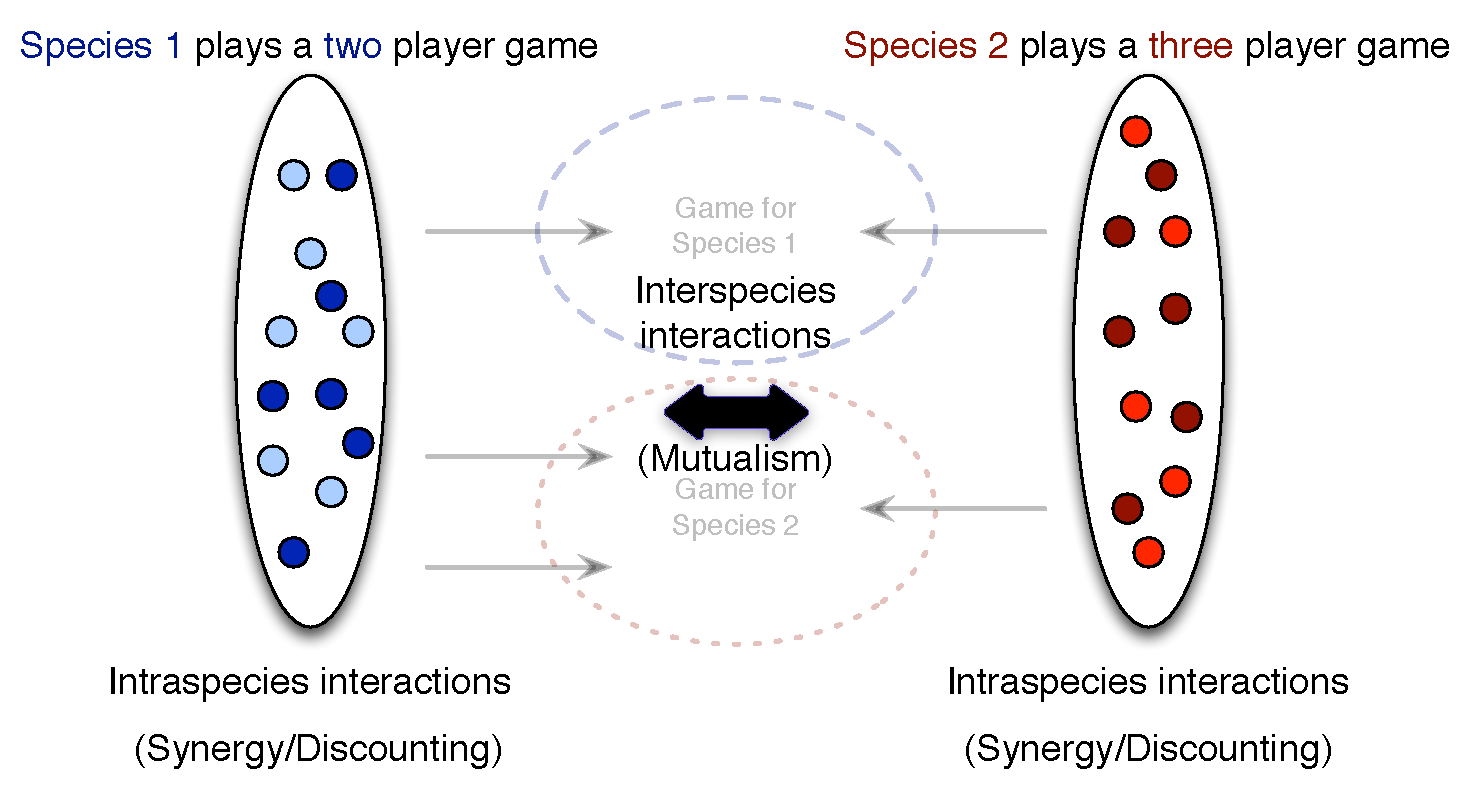
\includegraphics[scale=0.5]{../Figures/interintra.pdf}
\caption{\small{
\textbf{Evolutionary dynamics with combined inter-intra species dynamics.}
We assume the interactions between species to be mutualistic described by the snowdrift game \citep{bergstrom:PNAS:2003,souza:JTB:2009,gokhale:PRSB:2012}.
Species $1$ plays a $d_1^{inter}$ player game with Species $2$ while Species $2$ plays a $d_2^{inter}$ player game.
Each species has two types of players ``Generous" and ``Selfish" who besides interacting with the members of other species, also take part in intra species dynamics.
\cha{We assume a general framework of synergy and discounting for the intraspecies interactions \citep{eshel:AmNat:1988,hauert:JTB:2006a}
}}
\marcus{Would it be good to include something like ``proportion of generous: $x$'' on the left/blue side of the figure at the bottom, and ``proportion of generous: $y$'' on the right?}
\label{fig:conceptart}
}
\end{center}
\end{figure}


\subsection{Interaction dynamics}
\subsubsection{Interspecies}

Since we focus on mutualism the interspecies dynamics is given by the multiplayer version of the snowdrift game \citep{bergstrom:PNAS:2003,souza:JTB:2009,gokhale:PRSB:2012} (also known as hawk-dove, or chicken).
In this, a common benefit is possible but there is a cost to contributing and species do not need to contribute equally. However the individuals in each species could get away with contributing a bit less than other individuals.
\marcus{Awkward wording I think, but I haven't fixed yet.}
Hence for example if producing brighter light comes at a premium for the \textit{Vibrio} in the squid then the dimmer \textit{Vibrio} would be better off (Note that not producing any light is not an option as it results in eviction).
We assume that each species consists of two types of individuals ``Generous" $G$ and ``Selfish" $S$. 
If enough individuals are ``Generous" and contributing to the generation of mutual benefits then other individuals can get away with being selfish (not contributing). But all individuals in the game lose out if not enough are generous. Hence both species cannot be completely ``selfish", as per the definition of mutualism.
This interaction framework corresponds to that of a multi player version of a snowdrift game and is discussed in detail in the Supplementary Material (SI).
Hence the pressure is on a species to make the partner ``Generous" while getting away itself by being ``Selfish".
The fitness of each of the types within a species thus depends on the composition of the other species.
Denoting the frequency of the``Generous" types in Species $1$ ($G_1$) as $x$, and that in Species $2$ ($G_2$) as $y$, the fitness of $G_1$  is given by $f^{inter}_{G_1} (y)$ and that of $G_2$ as $f^{inter}_{G_2} (x)$. 

\subsubsection{Intraspecies}

For intraspecies dynamics we do not restrict ourselves to any particular interaction structure and thus can make use of the general multiplayer evolutionary games framework \citep{gokhale:PNAS:2010,gokhale:DGAA:2014}.
Moving from the interspecies dynamics, the two types already described are ``Generous" and ``Selfish".
Thus we already have each species containing two different types of individuals.
It is possible that a different categorisation exists within a species however for the sake of simplicity we study the dynamics between ``Generous" and ``Selfish" types within a species.
However the individuals which are ``Generous" for the interspecies interaction may/may not be more giving or in a sense ``Cooperators" for intraspecies dynamics.
Thus we need a flexible cost-benefit framework to model the intraspecies dynamics which can be easily tuned to the particular situation.
The cost benefit framework described in \citep{eshel:AmNat:1988,hauert:JTB:2006a}
 allows us to transition between four classic scenarios of evolutionary dynamics \citep{nowak:Science:2004}.
For example in our case we can have a dominance of the ``Generous" type or the ``Selfish" type or both the types can invade from rare resulting in a co-existence or bistability if both pure strategies are mutually non-invasive.
For the intra species interactions the fitness of a $G_1$ is then given by $f^{intra}_{G_1} (x)$ and that of $G_2$ is given by $f^{intra}_{G_2} (y)$ and similarly for the ``Selfish" types.

\subsection{Combined dynamics}

Putting together intra and interspecific dynamics provides a complete picture of the possible interactions occurring. While we are interested in mutualism at the level of the interspecies interactions there are four possible interactions within each species \citep{nowak:Science:2004,hauert:JTB:2006a} \marcus{(briefly spell them out here, I think)}. Since the within species interactions for the two different species do not need to be the same, there are in all sixteen different possible combinations.
Assuming additivity in the fitnesses of inter and intraspecies fitnesses, the combined fitness of each of the two types in the two species are given by,

%
\begin{align}
	f_{G_1} (x,y) &= p f^{inter}_{G_1} (y) + (1-p) f^{intra}_{G_1} (x) \nonumber \\
	f_{S_1} (x,y) &= p f^{inter}_{S_1} (y) + (1-p) f^{intra}_{S_1} (x) \nonumber \\
	f_{G_2} (x,y) &= p f^{inter}_{G_2} (x) + (1-p) f^{intra}_{G_2} (y) \\
	f_{S_2} (x,y) &= p f^{inter}_{S_2} (x) + (1-p) f^{intra}_{S_2} (y) \nonumber
\end{align}
%
The parameter $p$ tunes the impact of each of the interactions on the actual fitness that eventually drives the evolutionary dynamics.
For $p=1$ we recover the well studied case of the Red King dynamics \citep{gokhale:PRSB:2012} of the snowdrift game, while for $p=0$ the dynamics of the two species are essentially decoupled and can be individually studied by the synergy/discounting framework of nonlinear social dilemmas \citep{hauert:JTB:2006a}.
Our interest here is in the continuum and the intermediate values of $p$.
However that means we need to track the qualitative dynamics of sixteen possible intraspecies dynamics as $p$ changes gradually from close to $0$ to close to $1$ (SI). 
The time evolution of the ``Generous" types in both species is then given by,

\begin{align}
\dot{x} &= r_x x \left(f_{G_1}(x,y) -  \bar{f}_1(x,y) \right) \nonumber \\
\dot{y} &= r_y y \left(f_{G_2}(x,y) -  \bar{f}_2(x,y) \right).
\label{eq:repeqs}
\end{align}


This approach provides us with a powerful method to incorporate a multitude of realistic concepts in the analysis.
For example the number of players involved in a game, which has been shown to be a crucial factor in determining the evolutionary dynamics could be different for each interactions, inter and intra species interactions for Species $1$ ($d^{inter}_1$, $d^{intra}_1$) and similarly for Species 2 ($d^{inter}_2$, $d^{intra}_2$). 
The interspecies interactions are proxied by the multiplayer Snowdrift game which can incorporate threshold effects.
For example a certain number of ``Generous" cleaner fish may be required to clean the host or a certain number of ``Generous" ants required to protect larva from predators.
We can have $M_1$ and $M_2$ as the thresholds in the two species.
Since the interaction matrices for the inter and intra species dynamics are completely different in principle we can have different costs and benefits for the four games (Two snowdrift games from the perspective of each species and the intragames within each species).

We can have a diverse and rich set of dynamics possible which brings into question the study of coevolution based on only interspecies interactions. 
For the full spectrum of possible dynamics see Figure \ref{fig:appendix}.
As 
Even if we make a large number of assumptions and even if the intraspecies dynamics accounts for only $33\%$ ($1-p$) of the cumulative fitness, we can see drastically different qualitative dynamics which is capable of explaining the persistence of exploiters.

\begin{figure}
\begin{center}
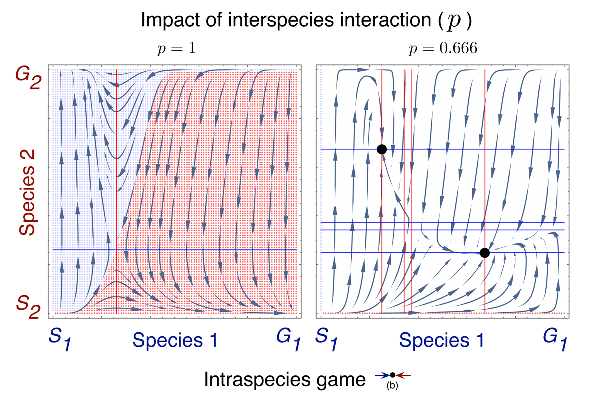
\includegraphics[width=\columnwidth]{../Figures/mainexample2.pdf}
\caption{\small{
\textbf{Change in evolutionary dynamics due to inclusion of intraspecies dynamics.} When the fitness of the ``Generous" and ``Selfish" types in both the species is solely determined by the interactions which occur between species (in this case mutualism, $p=1$) then we recover the dynamics as studied previously in \citep{gokhale:PRSB:2012}. The colours represent the initial states which result in an outcome favourable for Species $1$ (blue leading to ($S_1$,$G_2$)) and Species $2$ (red, leading to ($G_1$,$S_2$)). This can result in the red King effect and other possible complexities as discussed recently in \citep{gao:SciRep:2015}. However when we start including intraspecies dynamics the picture can be very different.
Even when the impact of intraspecies dynamics is only a $1/3$ on the total fitness of the ``Generous" and ``Selfish" types we see a very qualitatively different picture.
Two fixed points are observed where both the ``Generous" and ``Selfish" types can co-exist in both the species.
All initial states in the interior lead to either one of these fixed points (hence the lack of colours).
However it is still possible to characterize the ``successful" species as one of the equilibrium is favoured by one species than the other.
The horizontal isoclines are for Species $1$ while the vertical ones are for Species $2$.
The analysis was done for a 5 player game $d_1^{inter} = d_2^{inter} = d_1^{intra} = d_2^{intra} = 5$, $b=2$, $c=1$ and $r_x = r_y /8$ for the interspecies mutualism game while additionally $\tilde{b}_1 = \tilde{b}_2 = 10$ and $\tilde{c}_1 = \tilde{c}_2 = 1$ and $\omega_1 = \omega_2 = 3/4$ for the two intraspecies games within each species. Note that even with symmetric games within each species we can a qualitatively drastic difference when compared to the dynamics excluding intraspecies interactions.  For different intraspecies interactions within each species and for varying $p$ see SI.}
\label{fig:mainexampleone}
}
\end{center}
\end{figure}

\subsection{Population dynamics}

Until now we have considered that each species consists of two types of individuals and they make up the population of that species.
However populations sizes change over time. 
Assuming that ecological changes are fast enough that they can be averaged out, we can usually ignore their effect on the evolutionary dynamics.
It is now possible to show that evolution can happen at fast timescales, comparable to those of the ecological dynamics \cha{add citations with examples}.
Hence we need to tackle not just evolutionary but eco-evolutionary dynamics together.
%
\begin{figure}
\begin{center}
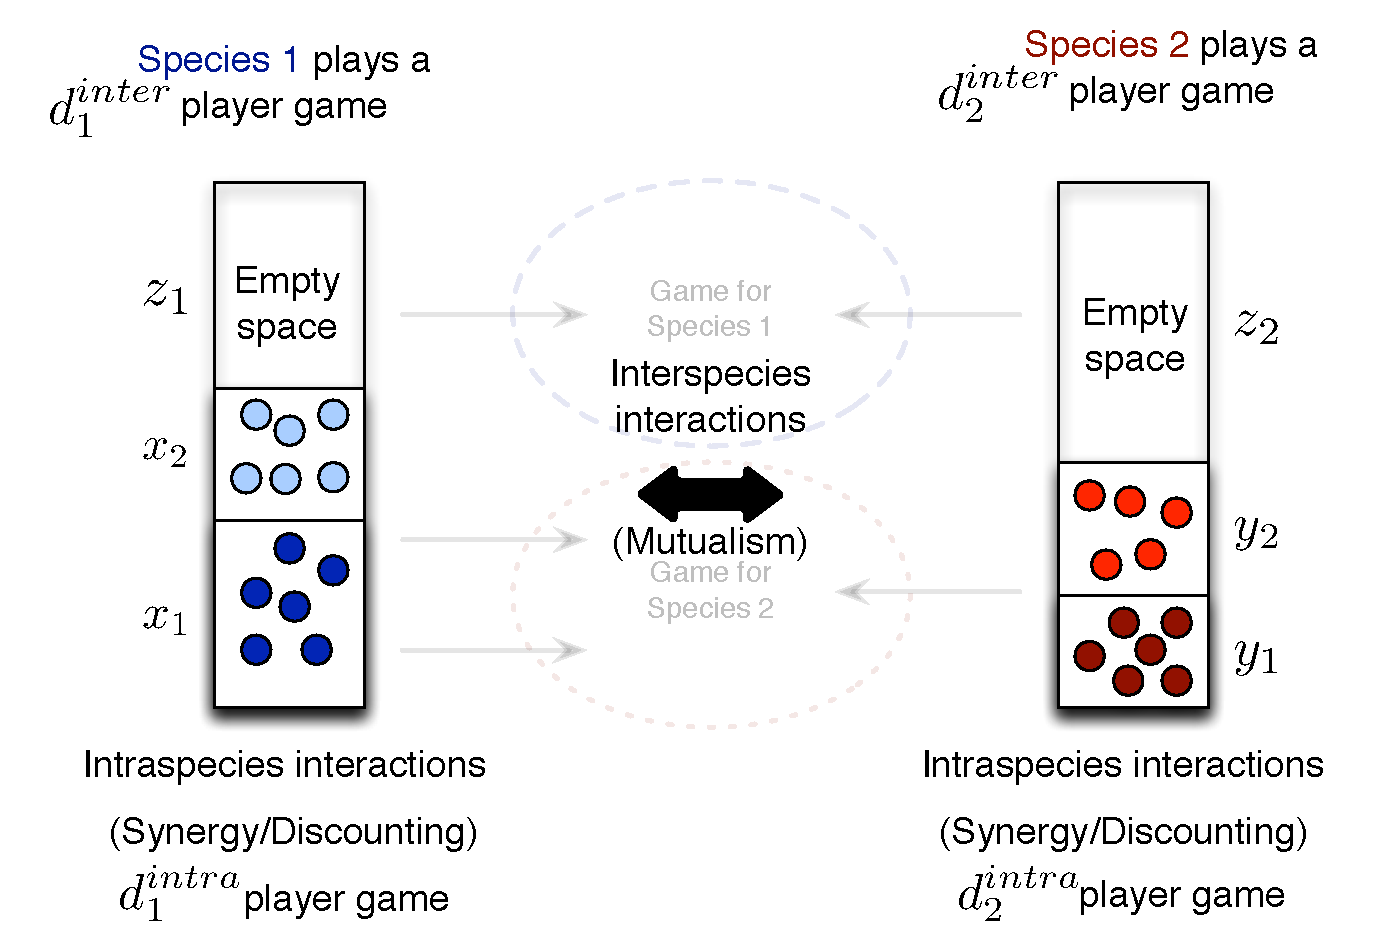
\includegraphics[scale=0.5]{../Figures/popdyninterintra.pdf}
\caption{\small{
\textbf{Population and evolutionary dynamics with combined inter-intra species dynamics.}
As with the interactions described in \ref{fig:conceptart} the two species consist of two types of individuals ``Generous" and ``Selfish".
Since the two species can in principle occupy different environmental niches, they  can have non-overlapping population carrying capacities.
The normalised carrying capacity in both species is $1$ and we have $x_1 + x_2 + z_1 = 1$ (for Species $1$) where $x_1$ and $x_2$ are the densities of the ``Generous" and ``Selfish" types respectively. 
The parameter $z_1$ represents the remaining space into which the population can still expand into.
For $z_1 = 0$ the population is at its carrying capacity while for $z_1 = 0$ Species $1$ is extinct. }
\label{fig:conceptartpopdyn}
}
\end{center}
\end{figure}
%

To include population dynamics in the previously considered scenario, we reinterpret $x_1$ now as the fraction of ``Generous" types and $x_2
$ as the fraction of ``Selfish" types in Species $1$.
Also now we have $z_1 = 1 - x_1 - x_2$ as the empty spaces in the niche occupied by Species $1$. Similarly we have $y_1$, $y_2$ and $z_2$ (Fig.~\ref{fig:conceptartpopdyn}).
This approach has previously been explored in terms of social dilemmas in \citep{hauert:PRSB:2006}.
We adapt and modify it for the two species and hence now the dynamics of this complete system is determined by the following set of differential equations,
%
\begin{align}
	\dot{x_1} &= r_x x_1 (z_1 f_{G_1} - e_1) \nonumber \\
	\dot{x_2} &= r_x x_2 (z_1 f_{S_1} - e_1) \\
	\dot{z_1} &= - \dot{x_1} - \dot{x_2} \nonumber
\end{align}
%
and for species 2
\begin{align}
	\dot{y_1} &= r_y y_1 (z_2 f_{G_2} - e_2) \nonumber \\
	\dot{y_2} &= r_y y_2 (z_2 f_{S_2} - e_2) \\
	\dot{z_2} &= - \dot{y_1} - \dot{y_2} \nonumber
\end{align}
%
where we have introduced $e_1$ and $e_2$ as the death rates of the two species.
Setting $e_1 = \frac{z_1 (x_1 f_{x_1} + x_2 f_{x_2}) }{x_1 + x_2}$ and $e_2 = \frac{z_2 (y_1 f_{G_2} + y_2 f_{S_2}) }{y_1 + y_2}$ we recover the two species replicator dynamics as in Eqs.~\ref{eq:repeqs} (For the sake of brevity we avoid showing the fitnesses in their the functional forms).
In this setup however the fitnesses need to be re-evaluated as not we need to account for the presence of empty spaces (See SI).
The dynamics is simplified by focusing on the proportion of ``Generous" types in both the species thus $g_1 = x_1/(1-z_1)$ and $g_2 = y_1/(1-z_2)$ whose time evolution is given by,
\begin{align}
	\dot{g_1} &= r_x z_1 g_1 (1-g_1) (f_{G_1} - f_{S_1}) \nonumber \\
	\dot{z_1} &= e_1 (1-z_1) - r_x z_1 (1-z_1) (g_1 f_{G_1} -  (1-g_1) f_{S_1})
\end{align}
and
\begin{align}
	\dot{g_2} &= r_y z_2 g_2 (1-g_2) (f_{G_2} - f_{S_2}) \nonumber \\
	\dot{z_2} &= e_2 (1-z_2) - r_y z_2 (1-z_2) (g_2 f_{G_2} -  (1-g_2) f_{S_2})
\end{align}
%
where everywhere we have $x_1 = g_1 (1-z_1)$ (with $x_2 = (1-g_1) (1-z_1)$) and $y_1 = g_2 (1-z_2)$ (with $y_2 = (1-g_2) (1-z_2)$) in the fitnesses as well.

Such a two species multi-type interaction system is a complicated as well as a realistic depiction of most of the mutualisms observed in nature.
However even with this complexity, the reduction of variables from six to four allows us to study the eco-evolutionary dynamics of the mutualism by looking at the two species simultaneously.
We take the most stable situation observed in the dynamics without population dynamics (Fig.~\ref{fig:mainexampleone}) which shows two internal stable equilibria and add population dynamics to it.
The results are summarized in Figure \ref{fig:popdyn} where we plot the evolutionary parameter (fraction of ``Generous" in each species) against the ecological parameter, the population density (or rather in this case the empty spaces) .

\begin{figure}
\begin{center}
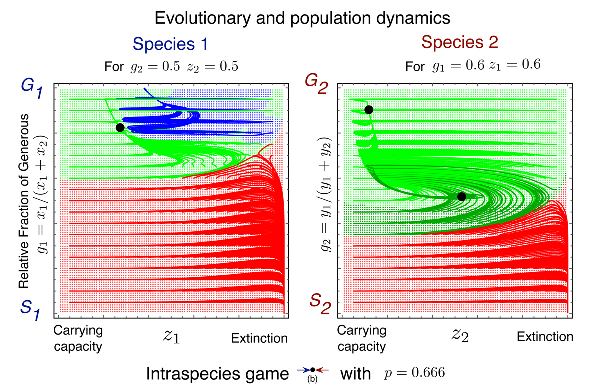
\includegraphics[width=\columnwidth]{../Figures/mainexamplepopdyn2.pdf}
\caption{\small{
\textbf{Dynamics of evolutionary strategies and population density for an intraspecies coexistence game with interspecies mutualism.}
With exactly the same parameters as that of Figure \ref{fig:mainexampleone} with  symmetric death rates $e_1 = e_2 = 0.05$ we show two different numerically evaluated examples.
Left Panel: shows the outcomes in Species $1$ when starting from $0.5$ fraction of ``Generous" individuals in Species $2$ at half carrying capacity $z_2 = 0.5$.
While most of the initial conditions lead to an extinction of Species $1$ (red), there exists a fixed point which can be reached when most of Species $1$ is ``Generous" and close to carrying capacity (green). For the same or higher fraction of $G_1$ but lower population density, Species $1$ can end up being completely ``Generous" (blue).
Right Panel: shows the outcomes in Species $2$ when starting from $0.6$ fraction of ``Generous" individuals in Species $1$ with empty spaces proportion of $z_1 = 0.6$.
When Species $2$ is mostly made up of ``Selfish" types then it leads to species extinction (red), For intermediate levels of ``Generous"individuals there exists an internal equilibrium (dark green). However another stable equilibrium exists as well as even higher densities of ``Generous" types closer to full carrying capacity (green).
Equilibrium selection is thus possible for Species $2$ in this case where it is preferable to have an intermediate number of ``Selfish" types.
\label{fig:popdyn}
}
}
\end{center}
\end{figure}

\subsection{Seasonality}

Mutualism may be only possible when the conditions for both the species are right to proliferate.

\section{Discussion}

Usually when interspecies relationships such as mutualism (or antagonist relationships as in predator-prey) are considered, the within species interactions are ignored for the sake of convenience. 
Obviously this is an assumption which is very useful when distilling the interactions at different community scales.
However when such interactions are interdependent then the connectivity between the different levels cannot be ignored \cite{Schluter:2012hn}.
As an example we focus on mutualism.
A fragile balance of parameters maintains mutualism.
Including realistic phenomena such as intraspecies interactions, population dynamics and seasonality we show that maintenance of mutualism is possible.
However often it can come at a cost of maintaining a significant level of exploiters as well.
In fact the coevolutionary dynamics between the two species is determined together by the inter as well as the intraspecific interactions.

In our study we have mutualistic interactions between two species. This can be represented by a bimatrix game. The components of each of the bimatrix game need not be correlated as long as they satisfy the inequalities leading to a Snowdrift games.

\textbf{Acknowledgements}. Thanks for all the fish.


\bibliographystyle{plainnat}
%\bibliographystyle{mdpi}

\bibliography{\string~/Bibtex/et.bib}

\renewcommand{\theequation}{A.\arabic{equation}}
\setcounter{equation}{0}

\renewcommand{\thefigure}{A.\arabic{figure}}
\setcounter{figure}{0}

\begin{appendices}

\section{Interspecies Evolutionary Dynamics}

Traditional coevolutionary models consider interspecific dependence only \citep{roughgarden:TPB:1976,roughgarden:book:1983}.
Since in our case each the interactions between the Species are mutualistic and each Species consists of two types of individuals ``Generous" and ``Selfish", the following Snowdrift game is an appropriate representation of the interactions.
%This is because we have neglected intraspecific interactions as mentioned earlier.

%For different types of interactions between species differrent models need to be defined \citep{poulin:JTB:1995,doebeli:PNAS:1998,noe:book:2001,johnstone:ECL:2002,bergstrom:PNAS:2003,hoeksema:AmNat:2003,akcay:PRSB:2007,bshary:Nature:2008}.




\subsection*{The snowdrift game}
\label{appA}
\subsubsection*{Two player setting}
%So far, we have described general games within and between species, now we turn to a particular game which of interest to us when considering mutualism.
Two drivers are stuck in a snowdrift.
They must shovel away the snow (paying the cost $c$) to reach home (benefit $b$) but there are three possible outcomes to this scenario.
One of the driver shovels while the other stays warm in the care ($b-c$ and $b$), both the drivers share the workload and shovel away the snow ($b-c/2$ and $b-c/2$) or none of them gets out of the care and they both remain stuck ($0$ and $0$).

Putting this game in perspective of the two species (i.e. the two drivers represent the two different species) we get the matrix,\\
%
\begin{equation}\label{}
\begin{array}{cc|cc}
\multicolumn{4}{l}{\textit{Species 1 payoff:}} \\
\hline\hline
& & \multicolumn{2}{c}{\text{Species 2}}\\
&	&	G_2		&	S_2	\\
\hline
 \multirow{2}{*}{Species 1} & G_1 	& b-c/2 &	b-c \\
&	S_1	&  b & 0 \\
 \hline\hline
\end{array}
\hspace{1cm}
\begin{array}{cc|cc}
\multicolumn{4}{l}{\textit{Species 2 payoff:}} \\
\hline\hline
& & \multicolumn{2}{c}{\text{Species 1}}\\
&	&	G_1		&	S_1	\\
\hline
 \multirow{2}{*}{Species 2} & G_2 	& b-c/2 &	b-c \\
&	S_2	& b & 0 \nonumber \\
 \hline\hline
\end{array}
\end{equation}
%
where strategy $G$ stands for being \textit{``Generous"} and shoveling the snow while $S$ stands for being \textit{``Selfish"} and just sitting in the car.
For $b=2$ and $c=1$ we recover the matrix used in \citep{bergstrom:PNAS:2003}.

For the snowdrift game in a single population for which the pairings are formed at random, there exists a single, stable internal equilibrium.
Hence the population will evolve to a polymorphism which is a combination of \textit{``Generous"} and \textit{``Selfish"} individuals.
But in a two species system (pairs still random, but one from each species), this stable equilibrium turns into a saddle point: a small deviation from this fixed point leads the system to one of the stable fixed point where one of the species is completely \textit{``Generous"} and the other one is completely \textit{``Selfish"}.

\subsection*{Multiplayer setting}
\label{appB}

Following Souza et al. \citep{souza:JTB:2009},  
a multiplayer snowdrift game can be described by the payoff entries
\begin{eqnarray}
\Pi_{G_1} (k)  &=& \begin{cases} b-\frac{c}{k} & \textrm{if } k \geq M \\  -\frac{c}{M} & \textrm{if } k < M \end{cases}
\\
\Pi_{S_1} (k)  &=& \begin{cases} b & \textrm{if } k \geq M \\ 0 & \textrm{if } k < M. \end{cases}
\end{eqnarray}
%
All players get the benefit $b$ if the number of generous individuals in both species combined, $k$, is greater than or equal to the threshold $M$.
For the generous individuals, their effort is subtracted from the payoffs.
The effort is shared if the quorum size is met ($\frac{c}{M}$), but is in vain for $k<M$. \marcus{I'm confused here: why is $\frac{c}{k}$ lost if above the threshold but  $\frac{c}{M}$ lost if not?}
For two player games we had $k=1$ but multiplayer games provide the possibility of exploring this threshold aspect of collective action games.
From these payoff entries we need to calculate the average fitnesses.
For simplicity we just illustrate the fitnesses of the strategies in Species $1$.
For a $d_1^{inter}$ player game for Species $1$ we need to pick $d_1^{inter}-1$ other individuals from Species $2$.
Assuming random sampling the composition of the formed groups is given by a binomial distribution.
Summing over all possible compositions of groups we arrive at  the average fitnesses of the two strategies in species $1$,
%
\begin{align}
f^{inter}_{G_1} (y) &= \sum_{k=0}^{d_1^{inter} -1} \binom{d_1^{inter} -1}{k}y^k (1-y)^{d_1^{inter} -1-k} \Pi_{G_1}(k+1) \\
f^{inter}_{S_1} (y) &= \sum_{k=0}^{d_1^{inter} -1} \binom{d_1^{inter} -1}{k}y^k (1-y)^{d_1^{inter} -1-k} \Pi_{S_1}(k).
\label{interfiteqs}
\end{align}
%


\section{Intraspecies Evolutionary Dynamics}
\label{appB}

For elucidating the intraspecies dynamics we will focus on Species $1$ as the analysis is analogous for Species $2$.
Withing species dynamics can in principle be completely different from the between species interactions. 
We can have a multistrategy multiplayer game within a Species but to keep things simple we assume a two strategy multiplayer game.
The partitioning of the individuals into two strategies follows the same partitioning as in the inter species interactions as of ``Generous" and ``Selfish". 
However we can relabel them as ``Cooperators" and ``Defector" for the sake of the interactions structure which we will be making use of.
Note that the ``Generous" in the interspecies interactions need not always be the ``Cooperators" for the within species interaction but again for the sake of simplicity we will assume it  to be so. \marcus{Ah! now I get it. I guess we need to highlight this earlier on, as it's a strong condition: I found myself wondering whether Generous in inter $\leftrightarrow$ Cooperator in intra, or not...}

\subsection*{Synergy/Discounting Framework}
We model the within species interactions by making use of a general framework of costs and non-linear benefits \citep{eshel:AmNat:1988,hauert:JTB:2006a} which can potentially encompass all different types of (traditionally studied) social interaction structures qualitatively \citep{nowak:book:2006} \marcus{Perhaps good to list the 4 types}.
For Species $1$ the frequency of cooperators is just $x$ and the defectors is $1-x$, the same as the ``Generous" and ``Selfish". \marcus{Q: is this because they are the very same players? ie. are we assuming a Generous player in the inter is a Cooperative one in the intra?}
The ``Cooperators" and ``Defectors" in Species $1$ play a $d_1^{intra}$ player game.
Thus the fitnesses of cooperators and defectors are defined as \citep{hauert:JTB:2006a},
%
\begin{align}
	f^{intra}_{G_1} (x) &= \sum_{k=0}^{d_1^{intra} -1} \binom{d_1^{intra} -1}{k}x^k (1-x)^{d_1^{intra} -1-k} \Gamma_{G_1}(k+1) \\
	f^{intra}_{S_1} (x) &= \sum_{k=0}^{d_1 -1} \binom{d_1^{intra} -1}{k}x^k (1-x)^{d_1^{intra} -1-k} \Gamma_{S_1}(k).
\label{intrafiteqs}
\end{align}
%
where the payoffs are given by,
\begin{align}
	\Gamma_{S_1} (k) = \frac{\tilde{b}}{d_1^{intra}} \sum_{i=0}^{k-1} \omega^i \\
	\Gamma_{G_1} (k) = \Gamma_{S_1} (k) - \tilde{c}.
\label{eqintragamepayoffs}
\end{align}
%
Thus the defectors get a fraction of the benefit which is scaled by the factor $\omega$, which determines whether the benefits are linearly accumulating ($\omega=1$) for increasing number of cooperators, synergistically enhanced ($\omega>1$) or saturating ($\omega<1$).
Note that the costs and benefits in the within species game need not be the same as in between species ($b\neq \tilde{b}$ and $c \neq \tilde{c}$).


\section{Combined Evolutionary Dynamics}

The average payoffs are then just assumed to be a linear combination of the interspecies and intraspecies interactions where the parameter $p$ determines the strength of each of the interactions such that,
%
\begin{align}
	f_{G_1} (x,y) &= p f^{inter}_{G_1} (y) + (1-p) f^{intra}_{G_1} (x) \\
	f_{S_1} (x,y) &= p f^{inter}_{S_1} (y) + (1-p) f^{intra}_{S_1} (x)
\label{fiteqs}
\end{align}
%
Following the same procedure for the two strategies in species $2$ leads to the average fitness
%
\begin{align}
\bar{f}_1 (x,y) &= x f_{G_1} (x,y)+(1-x) f_ {S_1}(x,y)\\
\bar{f}_2 (x,y) &= y f_{G_2} (x,y)+(1-y) f_{S_2}(x,y).
\label{avgfiteqs}
\end{align}
%
The time evolution of the ``Generous" types in both the species will give us the complete dynamics of the system.
However since the two interaction species are by definition different organisms, they can have different rates of evolution.
Thus if species 1 evolves at the rate $r_x$ while species 2 at rate $r_y$ then we have,
\begin{align}
\dot{x} &= r_x x \left(f_{G_1}(x,y) -  \bar{f}_1(x,y) \right) \nonumber \\
\dot{y} &= r_y y \left(f_{G_2}(x,y) -  \bar{f}_2(x,y) \right).
\label{eq:repeqs}
\end{align}


\begin{figure}[h]
\begin{center}
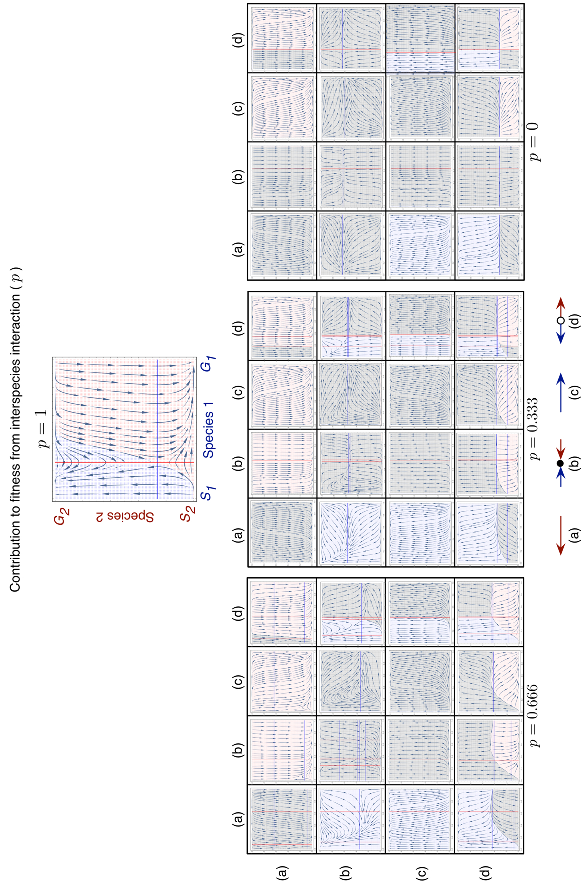
\includegraphics[width=\columnwidth]{../Figures/Dynamicsacrossp_reduced.pdf}
\caption{
$d_1^{inter} = d_2^{inter} = 5$, $b = 2$, $r_x = r_y/8$, $M_1 = M_2 = 1$ and $c=1$ for the interspecies game. As for the intraspecies games (a), (b), (c) and (d) the exact same parameter values as in \citep{hauert:JTB:2006a}.
\marcus{We need to spell out those 4 games at some point.}
\label{fig:appendix}
}
\end{center}
\end{figure}


\cha{\section*{Asymmetries}}

\cha{This between and within species model is a powerful way of introducing a lot of variability into the dynamics,
\begin{align}
	d_1 &\neq d_2 \\
	d^{inter} &\neq d^{intra} \\
	M_1 &\neq M_2 \\
	b &\neq \tilde{b} \\
	c &\neq \tilde{c} \\
	r_x &\neq r_y \\
	&\vdots
\end{align}
and various combinations of these. We should justify why we don't do this here and why we do vary the ones that we do.}


%\subsection{Dynamics in asymmetric conditions}
%
%%We have addressed two kinds of asymmetries in the game, the number of player and the thresholds in the two species.
%%We denote the number of players for species $1$ and species $2$ as $d_1$ and $d_2$, respectively, as in Fig.\ \ref{fig:counter}.
%%That is if species $2$ is playing a $d_2$ player game it means that one player from species $2$ interacts with $d_2-1$ players of species $1$.
%%For an asymmetry in the thresholds we use the two parameters $M_1\geq1$ and $M_2\geq1$ for the two species, respectively.
%
%For asymmetric bimatrix games, there is a difference in the dynamics between the standard replicator dynamics and the 
%alternative dynamics put forward by Maynard-Smith \citep{maynard-smith:1982to}.
%For this dynamics, the average fitness of each species appears as a denominator,
%\begin{align}
%\dot{x} &= r_x x \left(f_{G_1}(y) -  \bar{f}_1(x,y) \right)/\bar{f}_1(x,y) \nonumber \\
%\dot{y} &= r_y y \left(f_{G_2}(x) -  \bar{f}_2(x,y) \right)/\bar{f}_2(x,y).
%\label{eq:repeqs}
%\end{align}
%In our asymmetric bimatrix game, the fixed point stability is affected by the choice of the dynamics, in contrast to the case of symmetric games. 
%%In Fig.\ \ref{fig:thresholdsmodrep}, we illustrate that the dynamics is different between the usual replicator dynamics and Eqs. \ref{eq:repeqs}
%
%For $d_1=d_2 \geq 5$, the exact coordinates of the fixed point must be computed numerically \citep{abel:AO:1824,stewart:book:2004}.


\section{Population dynamics}

For brevity we begin with the description of population dynamics in Species 1.
The two types in Species 1, ``Generous" and ``Selfish" need not sum up to $1$ i.e. the population may not always be at its carrying capacity.
Hence if the empty space in the niche occupied by Species $1$ is $z_1$, then we have $x_1 + x_2 + z_1 = $ where $x_1$ and $x_2$ are the densities of ``Generous" and ``Selfish" types.
The population dynamics then is dictated by,
%
\begin{align}
	\dot{x_1} &= r_x x_1 (z_1 f_{G_1} - e_1) \\
	\dot{x_2} &= r_x x_2 (z_1 f_{S_1} - e_1) \\
	\dot{z_1} &= - \dot{x_1} - \dot{x_2}
\end{align}
%
and for species 2
\begin{align}
	\dot{y_1} &= r_y y_1 (z_2 f_{G_2} - e_2) \\
	\dot{y_2} &= r_y y_2 (z_2 f_{S_2} - e_2) \\
	\dot{z_2} &= - \dot{y_1} - \dot{y_2}
\end{align}
%
We have $e_1$ and $e_2$ as the death rates for the two species.
Setting $e_1 = \frac{z_1 (x_1 f_{x_1} + x_2 f_{x_2}) }{x_1 + x_2}$ and $e_2 = \frac{z_2 (y_1 f_{G_2} + y_2 f_{S_2}) }{y_1 + y_2}$ we recover the two species replicator dynamics as in Eqs.~\ref{eq:repeqs}. 
\marcus{This comes across as a special case only - justified? - or rephrase.}
The fitnesses however need to be reevaluated in this setup.
For example in Species 1 the fitness for type $G_1$ is,
%
\begin{align}
	f_{G_1}^{inter} &= \sum_{S=2}^{d_1} \binom{d_1 -1}{S-1} z_2 ^{d_1 -S} (1-z_2)^{S-1} P_G^{inter}(S,y_1,y_2,z_2) \\
	f_{G_1}^{intra} &= \sum_{S=2}^{d_1} \binom{d_1 -1}{S-1} z_1 ^{d_1 -S} (1-z_1)^{S-1} P_G^{intra}(S,x_1,x_2,z_1) \\
	f_{G_1} &= f_{G_1}^{inter} + f_{G_1}^{intra}
\end{align}
%
and similarly for type $S_1$ where the payoff functions are defined as,
%
\begin{align}
	P_G^{inter}(S,p,q,r) &= \sum_{k=0}^{S-1} V(S,p,q,r) \Pi_{G_1}(k+1) \\
	P_G^{intra}(S,p,q,r) &= \sum_{k=0}^{S-1} V(S,p,q,r) \Gamma_{G_1}(k+1) \\
	P_S^{inter}(S,p,q,r) &= \sum_{k=0}^{S-1} V(S,p,q,r) \Pi_{S_1}(k) \\
	P_S^{intra}(S,p,q,r) &= \sum_{k=0}^{S-1} V(S,p,q,r) \Gamma_{S_1}(k)
\end{align}
%
where $V(S,p,q,r) = \binom{S-1}{k} \left( \frac{p}{1-r}\right)^k  \left(\frac{q}{1-r}\right)^{S-1-k}$ is the probability of having a $k$ ``Generous"(Cooperator) individuals and $S-1-k$ ``Selfish"(Defector) individuals in the inter(intra) species game.
and the actual payoffs are calculated as per Eqs.~\ref{eqintergamepayoffs} and \ref{eqintragamepayoffs}.

\end{appendices}

\end{document}